% !TEX root = ../mat999.tex
\newpage
\section{Expectation}
Recall that a RV is a measurable function $X:(\Omega, \F)\mapsto (\bar{\R}, \bar{\B})$
\begin{dfn}[Expectation] The expectation (expected value/ mean) of RV $X$ defined on the probability space $(\Omega, \F, \prob)$ is \begin{equation*}
    \E(X) := \into X d\prob
\end{equation*}
Provided the integral is well-defined. \\
\textbf{Note:} $\E(X)$ is well-defined iff $\min(\E(X^+), \E(X^-)) < \infty$
\end{dfn}
Recall that for a RV X defined on $(\Omega, \F, \prob)$, we define $\mu_X$ the probability measure induced by $X$ on $(\bar{R}, \bar{\B})$ (push forward of $\prob$ under map $X$)
\begin{equation*}
    \mu_X(B) := \prob(\{\omega| X(\omega) \in B\}) \quad \forall B \in \bar{\B}
\end{equation*}

\begin{dfn}
    A RV $X$ on $(\Omega, \F, \prob)$ is \textbf{discrete} if $\exists \{x_k\} \subset \bar{\R} \text{ be countable}, x_k \neq x_l \text{ for } k\neq l$ s.t.
    \begin{align*}
        &\prob(X=x_k) = \mu_X(\{x_k\}) > 0 \\
        &\bigs{k} \prob(X=x_k) = \bigs{k}\mu_X(\{x_k\}) = 1
    \end{align*}
\end{dfn}we denote by $p(x) := \mu_X(x)$ the probability mass function of the RV X. The set $\{x|p(x)>0\}$ is called the support of the pmf of $\mu_X$
\begin{prop}
For a discrete RV $X$ with support $\{x_k\}$
\begin{enumerate}
    \item $\E(X)$ is defined $\Longleftrightarrow \min\{\bigs{k:x_k>0}x_kp(x_k),-\bigs{k:x_k<0}x_kp(x_k)\} < \infty$
    \item If $\E(X)$ is defined then 
    \begin{equation*}
        \E(X) = \bigs{k}x_kp(x_k)
    \end{equation*}
    \item $X\in \ls{1} \Longleftrightarrow \E(\abs{X})<\infty \Longleftrightarrow \bigs{k}\abs{x_k}p(x_k) < \infty$
    \item For any measurable function, $h: \bar{\R} \mapsto \bar{\R}$ the RV $Y = h(X)$ is discrete and 1-3 hold with $Y$ and $h(x_k)$
\end{enumerate}
\end{prop}
\begin{example}
If $h(x) = \sin(x)$ then $\E(\sin(X)) = \bigs{x} \sin(x_k) p(x_k)$ if expectation for $X$ is well-defined
\end{example}
\pf First ignore the zero measure part:  Let $A_k:=X^{-1}(x_k) = \{\omega|X(\omega) = x_k\} $ and $X' := \bigs{k}x_k \I_{A_k}$ \\
Then $X'$ is a discrete RV and $X = X'$ a.s. Assume first $X \geq0$ a.e. $\implies X' \geq 0$ a.e. and we have the integral are equal:
\begin{equation*}
    \E(X) = \E(X') = \int \bigs{k}x_k \I_{A_k}d\prob
\end{equation*}
Let $X_n := \bigs{k=1}^n x_k \I_{A_k}, X_n\uparrow X'$ and by MCT:
\begin{align*}
    \E(X) &= \E(X') = \int X' d\prob = \int \biglim{n} X_n d\prob = \biglim{n} \int X_n d\prob = \biglim{n} \bigs{k=1}^n x_k \prob(A_k) = \bigs{k} x_k \prob(A_k)\\
    \E(X) &= \bigs{k} x_k \prob(A_k)
\end{align*}\qed
\newpage 
\begin{dfn}AC and pmf \\
    The probability measure induced by RV $X, \mu_X$ is \textbf{absolutely continuous (AC)} w.r.t Lebesgue's measure $\lambda$, if $\mu_X(\R) = 1$ and if $\exists f:(\R, \B) \mapsto ([0,\infty), \B)$ measurable s.t. 
    \begin{equation*}
        \forall B \in \B, \prob(X\in B) = \mu_X(B) = \int_B fd\lambda = \int_\R f \I_B d\lambda
    \end{equation*}f is called the \textbf{density} of induced measure $\mu_X$
\end{dfn}
\begin{thm}[Change of variables formula] Let $X$ be a RV on $(\Omega, \F, \prob)$ and induced measure $\mu_X$ be distribution of X
\begin{enumerate}
    \item suppose that $h: (\bar{\R}, \bar{\B})\mapsto (\bar{R}^+, \bar{\B}^+)$ is measurable,let $Y:=h(X)$ Then $Y$ is non-negative RV with
    \begin{equation*}
        \E(Y) = \int Y\diff\prob = \int h(X) \diff\prob  = \int_{\bar{\R}} h \diff\mu_X
    \end{equation*}
    \item If $h: (\bar{\R}, \bar{\B})\mapsto (\bar{\R}, \bar{\B})$ is measurable then for $Y = h(X)$
        \begin{enumerate}
            \item $\E(Y) = \int Y\diff \prob$ is defined iff $\int h \diff\mu_X$ is defined and then
            \begin{equation*}
                \E(Y) = \int h \diff \mu_X
            \end{equation*}
            \item $Y\in \ls{1}(\Omega,\F, \prob)$ iff $h\in \ls{1}(\bar{\R}, \bar{\B}, \mu_X)$
        \end{enumerate}
    \begin{rem}
    Part 1 and 2 holds for any RVs (discrete/ continuous/ singular ...)
    \end{rem}
    \item If $X$ has a density $f$ ,then 
    \begin{equation*}
        \E(Y) = \int_\R hf \diff\lambda
    \end{equation*}(Lebesgue integral) with $\E(Y)$ is defined iff $\int_\R hf \diff\lambda$ exists

    \item If $X$ has density $f$ and $h: \R \mapsto \R^+$ is measurable s.t. $g(x):= h(x)\cdot f(x)$ is Riemann integrable on any finite interval, then 
    \begin{equation*}
        \E(Y) = \int_\R fh \diff\lambda = \inti h(x)f(x) \diff x
    \end{equation*}
    \item Condition on $h$ in 4 and we generalise it to the case $\R \mapsto \R$ \\
    $\E(Y)$ is well-defined if $\min\{\inti h^+f(x) \diff x, \inti h^-f(x) \diff x\}<\infty$ and then we have:
    \begin{equation*}
        \E(Y) = \inti h(x)f(x) \diff x
    \end{equation*}
\end{enumerate}
\end{thm}
\pf 

\newpage
\begin{cor}
$X\in \ls{1}$ iff $\inti \abs{x}f(x) \diff x < \infty$
\end{cor}
\begin{cor}
If $X$ has a density $f$ s.t. $g(x)= xf(x)$ is Riemann integrable on any finite interval, then $E(X)$ is defined iff
\begin{equation*}
    \int_{-\infty}^0 x f(x) \diff x > -\infty \quad\text{or}\quad \int_{0}^\infty x f(x) \diff x < \infty
\end{equation*} and if defined then
\begin{equation*}
    \E(X) = \inti xf(x) \diff x
\end{equation*}
\end{cor}
\begin{rem}
This definition does not means the expectation is finite, only existence can be guaranteed
\end{rem}
\begin{prop}
Let $X_1, X_2$ be RVs on $(\Omega, \F, \prob)$
\begin{enumerate}
    \item If $X_n$ are uniformly bounded $(\abs{X_n}\leq c < \infty \quad a.s).$ and $X_n \rightarrow X$ a.s. then $X_n \rightarrow X$ in $\ls{1}$ \\
    Bounded Convergence Theorem
    \item If $X_i \in \ls{1}$ then $\E(\bigs{i=1}^n X_i) = \bigs{i=1}^n \E(X_i)$
    \item If $X\geq 0 $ a.s. then $\E(X) \geq 0$. Also if $X_i\geq 0$ a.s. $\E(\bigs{i=1}^\infty X_i) = \bigs{i=1}^\infty \E(X_i)$, this is always well defined
    \item If $\E(X) < \infty$ then $\prob(X < \infty ) = 1$
    \item If $X_n \geq 0$ a.s. and $\bigs{n=1}^\infty \E(X_n) < \infty$ then by 4, $\bigs{n=1}^\infty X_n < \infty$ a.s. and in particular, $X_n\xrightarrow{a.s.}0$
\end{enumerate}
\end{prop}
\newpage
\begin{prop}
Suppose $X$ is a measurable function defined on $(\Omega,\F, \mu)$ with $\mu(\Omega)<\infty$ Then
\begin{enumerate}
    \item if $X\in \ls{p}$ for $p\geq1$ then $X\in \ls{r}$ for $r \in [1,p]$ (i.e. $\ls{p}$ spaces are nested and it is not necessarily the case for infinite measure)
    \item If $\mu = \prob$, then $\norm{X}_r \leq \norm{X}_p$, for $p \geq r \geq 1$, that is existence of higher moment always imply existence of lower moment.
\end{enumerate}
\end{prop}
\pf If $p >1$ and $r\in [1,p)$, define $p' = \frac{p}{r} > 1$ then $\exists q' > 1 \quad \frac{1}{p'} + \frac{1}{q'} = 1$ Conjugate. and then we have (By Holder's inequality \ref{holder}):
\begin{align*}
    \norm{X}_r^r = \int \abs{X}^r \cdot 1 \diff\mu &\leq  \left(\int \abs{X}^{rp'}  \diff\mu\right)^{\frac{1}{p'}}\left(\int \abs{1}^{q'}  d\mu\right)^{\frac{1}{q'}} \\
    &=\left(\int \abs{X}^p \diff\mu\right)^{\frac{r}{p}}\mu(\Omega)^\frac{1}{q'} \\
    &= \norm{X}_p^r\mu(\Omega)^\frac{1}{q'} \\
    \implies \norm{X}_r &\leq  \norm{X}_p \mu(\Omega)^\frac{1}{rq'} \leq \infty
\end{align*}\qed
\newpage
\subsubsection*{convex function and Jensen's inequality}
\begin{figure}[h]
    \centering
    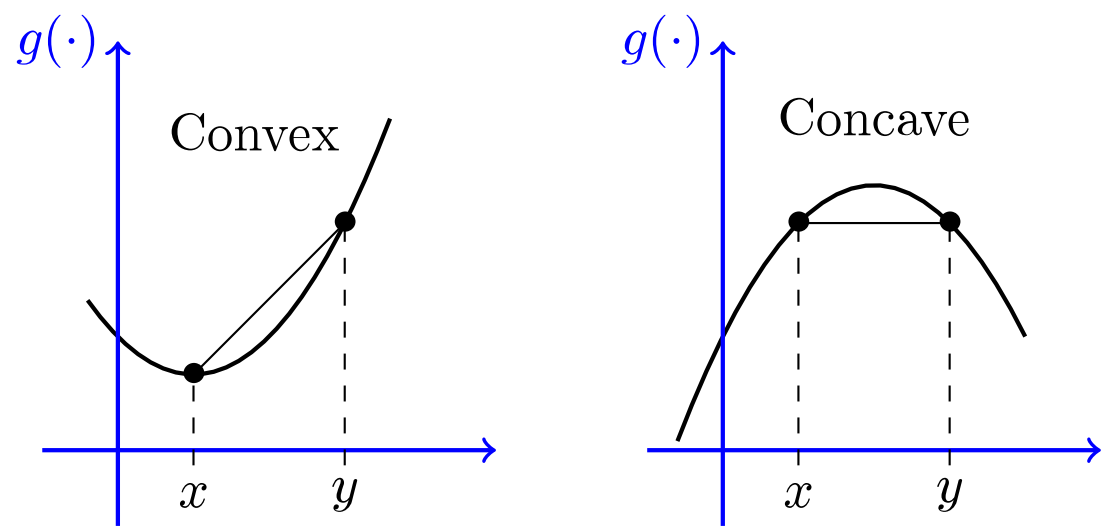
\includegraphics[scale = 0.2]{convex.png}
    \caption{Convex and concave function}
\end{figure}
\begin{dfn}[Convex function] A function $\phi: I \mapsto \R$ is convex on an open interval $I$ if $\forall x,y \in I$ and parameterise by $t\in(0,1):$
\begin{equation*}
    \phi(tx + (1-t)y)\leq t\phi(x) + (1-t)\phi(y), \quad \forall t \in (0,1)
\end{equation*}
\end{dfn}
\begin{lem}[Slope inequality]If $a < b < c \in I$ then we have \\
(Notation: $S([a,b]) := \frac{\phi(b) - \phi(a)}{b-a}$)
\begin{align*}
    &\frac{\phi(b) - \phi(a)}{b-a} \leq \frac{\phi(c) - \phi(a)}{c-a} \leq \frac{\phi(c) - \phi(b)}{c-b}   \\
    &S([a,b]) \leq S([a,c]) \leq S([b,c])
\end{align*}
\end{lem} Consider slope of the triangle formed by a,b,c:
\vspace{3cm}
\begin{cor}
Given convex function $\phi$, For any $x \in I$ left and right derivatives $D_{-\phi}$ and $D_{+\phi}$ exist and satisfy:
\begin{align*}
    D_{-\phi} := \biglim{h\rightarrow 0^+} \frac{\phi(x) - \phi(x-h)}{h} \leq \biglim{h\rightarrow 0^+} \frac{\phi(x+h) - \phi(x)}{h} =: D_{+\phi}
\end{align*}
\end{cor}
\vspace{3cm}
\begin{cor}
For any $x_0 \in I$ and $m\in [D_{-\phi}(x_0),D_{+\phi}(x_0)]$, we have:
\begin{equation*}
    m(x-x_0) + \phi(x_0) \leq \phi(x)
\end{equation*}$m(x-x_0) + \phi(x_0)$ is supporting line at $x_0$ of $\phi$
\end{cor}
\newpage
\pf of Lemma and Corollary on previous page
\newpage
\begin{thm}[Jensen's inequality]
\label{jensen}
If $\phi: I \mapsto \R$ is convex function on an open interval $I\subset \R$, and if $X$ is a RV in $\ls{1}$ with $\prob(X\in I)=1$, then $\E(\phi(X))$ is well-defined (possibly equal to $\infty$)
\begin{equation*}
    \E(\phi(X)) \geq \phi(\E(X))
\end{equation*}
\end{thm}

\pf Since $\prob(X\in I)=1$ and $X\in \ls{1}$, then $\E(X)$ exists and belongs to $I$. Let $x_0 = \E(X) \implies \forall y\in I$ we have \begin{align*}
    &m(y-\E(X))+\phi(\E(X)) \leq \phi(y) \\
    &\implies m(X-\E(X))+\phi(\E(X)) \leq \phi(X) \quad a.s. (*)\\
    &\implies \abs{\phi^-(X)} \leq K\abs{X} + c \quad \text{$\phi(X)$ is bounded below since $X \in \ls{1}$} \\
    &\implies \E(\phi(X)) \quad \text{is well defined} \\
    Integrate (*) \\
    &\E(m(X-\E(X))+\phi(\E(X))) \leq \E(\phi(X)) \\
    &\implies \E(m(X-\E(X))+\phi(\E(X))) = \phi(\E(X)) \leq \E(\phi(X))
\end{align*}\qed
\begin{rem}
Taking $\phi(x) = x^2$ be convex, then we have
\begin{equation*}
    \E(X^2) \geq \E(X)^2 \Longleftrightarrow \norm{X}_1 \leq \norm{X}_2
\end{equation*}
\end{rem}
\begin{ex}
Using Jensen's inequality to prove $\norm{X}_r \leq \norm{X}_p, r\in [1,p]$ 
\end{ex}
\newpage
\subsection*{Variance and Covariance}
If $X\in \ls{1}$ then $m := \E(X)$ is well-defined and finite. Since we have $(X-m)^2 = X^2 - 2mX + m^2$ then $(X-m)^2\in \ls{1}\Longleftrightarrow \E(X^2) < \infty \Longleftrightarrow X^2\in \ls{1} \Longleftrightarrow X\in \ls{2}$ Now:
\begin{dfn}[Variance of $X$]
\begin{equation*}
    V(X) := \E((X-m)^2) < \infty \Longleftrightarrow X\in \ls{2}
\end{equation*}
\end{dfn}
\begin{thm}[Chebyshev's Inequality]For $X\in \ls{2}$ with $m = \E(X)$
\begin{equation*}
    \prob(\abs{X-m}\geq \epsilon) \leq \frac{V(X)}{\epsilon^2}
\end{equation*}
\end{thm}
\pf Define $Y = (X-m)^2 \in \ls{1}$, By Markov inequality \ref{markov}
\begin{equation*}
\prob(Y\geq \epsilon) \leq \frac{\E(Y)}{\epsilon^2} =  \frac{V(X)}{\epsilon^2}   
\end{equation*}\qed
\begin{dfn}
For $X,Y\in\ls{1}$ with $X\cdot Y\in \ls{1}$ we define 
\begin{equation*}
    Cov(X,Y) := \E((X-m_X)(Y-m_Y))
\end{equation*}$m_X = \E(X) , m_Y = \E(Y)$
\end{dfn}Notice: $Cov(X,Y) = \E(X\cdot Y) - \E(X)\E(Y)$
\begin{dfn}[Non-correlated]
$\E(X\cdot Y) = \E(X)\E(Y) \Longleftrightarrow Cov(X,Y) = 0$
\end{dfn}
\begin{lem}
If $X_1,...,X_n \in \ls{2}$ then $X_k X_l \in\ls{1} \quad\forall k,l$ and \begin{equation*}
    V(\bigs{k=1}^n X_k) = \bigs{k=1}^n V(X_k) + \bigs{k\neq l}Cov(X_k,X_l)
\end{equation*}
\end{lem}
\pf If $k \neq l:$
\begin{equation*}
    \norm{X_k X_l}_1 \leq \norm{X_k}_2\norm{X_l}_2 < \infty
\end{equation*}By Holder's inequality \ref{holder},The rest are just binomial expansion \\

Generally $X,Y\in \ls{1}\notimplies X Y\in \ls{1}$ but this is the true if we add independency:
\begin{lem}If $X$ and $Y$ are independent, $X,Y\in \ls{1}$ then $X\cdot Y\in \ls{1}$ and
\begin{equation*}
    \E(XY) = \E(X)\E(Y)
\end{equation*}
\end{lem}
\begin{cor}Relation between independency and correlation 
\begin{enumerate}
    \item $Cov(X,Y) =0$ provided $X,Y$ independent
    \item If $X,Y\in \ls{2}$ and independent\begin{equation*}
        V(X+Y) = V(X) + V(Y)
    \end{equation*}
\end{enumerate}
\end{cor}
\newpage
\pf (a)The claim holds true if $X = \I_A$ and $Y = \I_B$, where $A,B\in \F$ and $A,B$ are independent events. \\
(b)$X = \bigs{k}\alpha_k \I_{A_k},Y = \bigs{l}\beta_l \I_{B_l}$ where $A_k, B_l\in \F, \alpha_k, \beta_l \geq 0$ note this is finite sum. \\
(c) $X,Y\geq 0 $, Let $X_n,Y_b$ be the setting as we did for Lebesgue integral, then we have two increasing and non negative sequence of RVs, by MCT
\begin{equation*}
    \E(X \cdot Y)\stackrel{MCT}{=} \biglim{n}\E(X_n Y_n) \stackrel{(b)}{=} \biglim{n} \E(X_n)\E(Y_n) = \biglim{n}\E(X_n) \biglim{n}\E(Y_n) \stackrel{MCT}{=} \E(X)\E(Y)
\end{equation*}Also we have
\begin{equation*}
    \E(X \cdot Y) = \E(X)\E(Y) < \infty \implies X \cdot Y \in \ls{1}
\end{equation*}
(d) Use the fact $X = X^+ - X^-,Y = Y^+ - Y^-$ and they are also independent. and $XY = X^+Y^+ +  X^-Y^- - X^+Y^- -  X^-Y^+$ and linearity of expectation.
\qed
\newpage
\subsection*{SLLN}
\begin{dfn}[A version of The strong law of large number]Suppose $X_i$ are i.i.d RVs with $\norm{X_i}_4 \leq c < \infty$, let $S_n := \bigs{i=1}^n X_i$. Then
\begin{equation*}
    \frac{S_n}{n} \xrightarrow{a.s.} m := \E(X_i)
\end{equation*}
\end{dfn}
\pf Step1: We may assume $m = \E(X_1) = 0$, otherwise, introduce \begin{equation*}
    X_i' := X_i - m, S_n' := \bigs{i=1}^n X_i' \implies \norm{X_i'}_4 \leq c + \abs{m}, S_n' = S_n - mn, \E(X_i') = 0
\end{equation*}. This is WLOG. \\
step2: Assuming $m=0$, \begin{equation*}
    S_n^4 = (\bigs{i=1}^n X_i)^4 = \bigs{i=1}^n X_i^4 + \bigs{i<j}\binom{4}{2} X_i^2X_j^2 + ... \text{The rest are all have terms with odd power}
\end{equation*}Every term is integrable given $\norm{X_i}_4  < \infty \implies S_n^4$ is integrable and take expectation.
\begin{align*}
    \E(S_n^4) &=  n \E(X^4) + 3n(n-1)\E(X^2)E(X^2) \\
    &= n\norm{X}_4^4+ 3n(n-1)\norm{X}_2^4 \\
    &\leq n c^4 + 3n(n-1)c^4 \leq 3n^2 c^4 \qquad(*) \\
    \E((\frac{S_n}{n})^4) &\leq 3c^4/n^2
\end{align*}Hence from (*): \begin{equation*}
    \E(\bigs{n\geq 1}(\frac{S_n}{n})^4) = \bigs{n\geq 1} \E((\frac{S_n}{n})^4) \leq \bigs{n\geq 1} \frac{3n^2c^4}{n^4} < \infty \implies (\frac{S_n}{n})^4 \xrightarrow{a.s.} 0 \implies \frac{S_n}{n} \xrightarrow{a.s.} 0
\end{equation*}\qed









\newpage
\section{Product measure}
Let $(\Omega_1, \F_1)$ and $(\Omega_2, \F_2)$ be measurable spaces, and let $\Omega:= \Omega_1 \times \Omega_2$ be their Cartesian product $(\Omega = \{(\omega_1, \omega_2)|\omega_i \in \Omega_i\})$ Let $\tau:= \{A_1 \times A_2 | A_i\in \F_i\}$.The $\tau$ is a $\pi$-system (intersection of rectangle is again rectangle) and we define:
\begin{equation*}
    \F := \sigma(\tau)
\end{equation*}$\F$ is called the product $\sigma$-algebra, and denoted $\F_1 \times \F_2$
\begin{rem}
$\F_1 \times \F_2$ is \textcolor{red}{Not} Cartesian product.
\end{rem}
Actually, $\tau$ is the Cartesian product.
\begin{ex}
Show the following results.
\begin{enumerate}
    \item Verify $\tau$ is a $\pi$-system
    \item Define $\rho_i : \Omega \mapsto \Omega_i$ as $\rho_i(\omega_1, \omega_2) = \omega_i$ The i-th coordinate map, Show that $\rho_i$ is $\F$ measurable.
    \item Show that $\F = \sigma(\rho_1,\rho_2)$ or equivalently $\F = \sigma(\{B_1\times \Omega_2, \Omega_1\times B_2|B_i \in \F_i \})$
\end{enumerate}
\end{ex}
\begin{rem}
\textbf{Both ways to define $\F$ work for a countable product of measurable spaces.}
\end{rem}This is important for stochastic process $X$ indexed by time. \\[0.5cm]
\textbf{Main issue} If $f: (\Omega, \F) \mapsto (\bar{\R}, \bar{\B})$ measurable, does it imply that 
\begin{align*}
    \forall \omega_1 \in \Omega_1, f(\omega_1, \cdot): (\Omega_2, \F_2) \mapsto (\bar{\R}, \bar{\B}) \\
    \forall \omega_2 \in \Omega_2, f(\cdot,\omega_2): (\Omega_1, \F_1) \mapsto (\bar{\R}, \bar{\B})
\end{align*} are measurable ? \textcolor{red}{Yes}

\begin{thm}[The Monotone Class Theorem]
\label{Monotonclass} Let $\M$(monotone class) be a class of bounded (not necessarily measurable) functions $\Omega \mapsto \R$ s.t. 
\begin{enumerate}
    \item $\M$ is a vector space over $\R$
    \item $\I_\Omega \in \M$
    \item If $(f_n) \in \M$ satisfy: $0\leq f_n\leq c <\infty$ and $f_n \uparrow$, then we have$\biglim{n\rightarrow\infty}f_n \in \M$
\end{enumerate}
If $\setp \subset \Omega$ is a $\pi$-system, and $\forall A \in \setp: \I_A \in \M$ then $\M$ contains every bounded $\sigma(\setp)$ measurable function
\end{thm}
\newpage
\pf Let $\setl :=\{A\subset\Omega| \I_A \in \M\}$
\begin{enumerate}
    \item $\I_\Omega \in \M \implies \Omega \in \setl$
    \item If $A,B \in \setl, A\subset B$ we have $\I_A, \I_B \in \M$ also $\I_{B\setminus A} = \I_B - \I_A \in \M$ since $\M$ is a vector space, Hence $\I_{B\setminus A}\in \M \implies B\setminus A \in \setl$
    \item Let $A_n\in \setl$ and $A_n \uparrow A$, Obviously $\I_{A_n} \leq 1< \infty$ and $\I_{A_n} \uparrow$ then we have \begin{equation*}
        \biglim{n\rightarrow\infty}\I_{A_n} = \I_{\biglim{n\rightarrow\infty}A_n} \in \M \implies A\in \setl
    \end{equation*}
\end{enumerate}Hence, $\setl$ is a $\lambda$-system. Since $\setp \subset \setl$ By Dynkin's theorem \ref{Dynkin} $\sigma(\setp) \subset \setl$ \\
But $\M$ is a vector space $\implies $ any bounded simple functions over  $\sigma(\setp)$ is in $\M$.\\
For any $f$ which is $\sigma(\setp)$ measurable and bounded, $\exists M < \infty, 0 \leq f \leq M < \infty$ and non-negative, Define
\begin{equation*}
    f_n := \bigs{k=1}^{n 2^n} \frac{k-1}{2^n} \I_{\{\frac{k-1}{2^n} \leq f \leq \frac{k}{2^n}\}} + n \I_{\{f\geq n\}}
\end{equation*}$f_n \in \M$ as it is a simple bounded $\sigma(\setp)$-measurable function, also $0\leq f_n \leq M$ and $f_n \uparrow f$, so $f \in \M$ by property 3 of $\M$ \\
Finally, any $\sigma(\setp)$-measurable function with $\abs{f}\leq M < \infty$ can be written as $f = f^+ - f^-$ and $f^+, f^- \in \M$ since they are measurable, bounded, non-negative. Again, $f = f^+ - f^-$ since $\M$ is a vector space.
\begin{rem}[Boundness of $f\in \M$] This makes the proof less technical, but this is not necessary.
\end{rem}
\begin{prop}\label{mesurability}
Let $f:(\Omega, \F) \mapsto (\bar{\R}, \bar{\B})$ be measurable, then 
\begin{align*}
 (*)\begin{cases}
   \forall \omega_1 \in \Omega_1, f(\omega_1, \cdot): (\Omega_2, \F_2) \mapsto (\bar{\R}, \bar{\B}) \\
    \forall \omega_2 \in \Omega_2, f(\cdot,\omega_2): (\Omega_1, \F_1) \mapsto (\bar{\R}, \bar{\B})
\end{cases}
\end{align*} are measurable
\end{prop}
\pf Let $\M :=\{ f:\Omega\mapsto\R, \text{f is bounded and (*) holds}\}$Then \begin{enumerate}
    \item $\M$ is a vector space over $\R$ \\
    If $f,g\in \M, a,b\in \R$ then $af+bg \in \M$ since linear combinations of bounded function is bounded same for measurability.
    \item $\I_\Omega \in \M$ obviously.
    \item If $(f_n) \in \M$ satisfy $ 0<(f_n)\leq c < \infty$ and $f_n \uparrow$, then $\biglim{n} f_n \in \M$ (limit exist because bounded convergent sequence, and limit of measurable functions are measurable)
\end{enumerate}Denote $\tau:= \{A_1 \times A_2 | A_i\in \F_i\}$, $\I_A \in \M$ since $\forall A\in \tau, \I_A{(\omega_1, \omega_2)} = \I_{A_1}(\omega_1)\cdot \I_{A_2}(\omega_2)$ which is clearly bounded, and if we restrict one coordinate, it it either 0 or indicator function of the other coordinate which is measurable.\\
Plus $\tau$ is a $\pi$-system shown is the previous exercise, therefore by Monotone Class theorem \ref{Monotonclass}:
\begin{equation*}
    \{\text{all bounded $\F$-measurable functions} \subset \M\}
\end{equation*}Note $\sigma(\tau) = \F$ 
\newpage
\textbf{Recall:}
\begin{thm}[Fubini–Tonelli theorem for Riemann integral]
If $f:\R^2 \mapsto\R^+$ is continuous, then with $I = [a,b], J = [c,d]$ where $a<b, c<d$ 
\begin{equation*}
    \iint_{I\times J} f(x,y) \diff x\diff y = \int_I \int_J f(x,y) \diff y\diff x = \int_J \int_I f(x,y) \diff x\diff y
\end{equation*}\rightline{LHS: double integral, RHS: iterated integral.} \\
The same holds for $f:\R^2 \mapsto\R$ continuous provided
\begin{equation*}
    \iint \abs{f} \diff x\diff y < \infty
\end{equation*}
\end{thm}
We have analogous result in the product space for Lebesgue's integral, but we need to define the analogue of double integral (Measure on the product space).\\
For Riemann integral, the double integral is defined in terms of Riemann sums w.r.t a 2-d lattice of rectangles. The contribution of each rectangle is 
\begin{equation*}
    f(x_i, y_i)\abs{R_{ij}} \qquad (x_i, y_i)\in R_{ij}, \quad \abs{R_{ij}}=\text{Area of }R_{ij}
\end{equation*}
The Lebesgue analogue would be to integrate on $\Omega_1\times \Omega_2$ with the "product measure" 
\begin{equation*}
    \mu(A_1 \cdot A_2) = \mu(A_1) \cdot \mu(A_2) \text{where }A_i\in\F_i
\end{equation*}
\begin{rem}
This definition is defined on the $\pi$-system which is $\tau$, but we have to extend it to the whole product $\sigma$-algebra
\end{rem}
We can define this product measure starting with the "rectangle" $A_1 \cdot A_2$ above then extending it using the Carathéodory's machinery.But since we have no idea what result measure we want, However, Fubini's theorem suggest an alternative approach (easier to calculate the measure of a complicated $A\in \F$) using the iterated integrals.
\newpage
\textbf{Setup:} Assume $\mu_i$ are finite measure no $(\Omega_i, \F_i), i=1,2$. Let $f: (\Omega, \F) \mapsto (\R, \B)$ be bounded and measurable and $\mu_i(\Omega_i) < \infty$
\begin{dfn}
The functions 
\begin{align*}
    I_1(\omega_1, f) := \int_{\Omega_2} f(\omega_1, \omega_2) \diff \mu_2 (\omega_2) \\
    I_2(\omega_2, f) := \int_{\Omega_1} f(\omega_1, \omega_2) \diff \mu_1 (\omega_1)
\end{align*}are well defined from $\Omega_i \mapsto \R$ follow the proposition \ref{mesurability}
\end{dfn}
\begin{lem}If $f:(\Omega, \F) \mapsto (\R, \B)$ is bounded and measurable then 
\begin{align*}
(**)\begin{cases}
    (i)\quad& \text{For } i=1,2: I_i(\cdot, f): (\Omega_i, \F_i) \mapsto (\R, \B) \text{ is bounded and measurable} \\
    (ii)\quad& \text{Fubini:} \int_{\Omega_1} I_1(\cdot, f) \diff \mu_1 = \int_{\Omega_2} I_2(\cdot, f) \diff \mu_2
\end{cases}
\end{align*}
\end{lem}
The proof is on next page
\begin{rem}We can extend above result to more general case ($\sigma$-finite)
\begin{enumerate}
    \item By replacing (i) in the above lemma by \\
    (i')$\text{For } i=1,2: I_i(\cdot, f): (\Omega_i, \F_i) \mapsto (\R, \B) \text{ is measurable}$ \\
    The lemma can be extended to $\sigma$-finite measures $\mu_i$ and $f \geq 0$, so (i')(ii) holds
    \item If follows that if $\mu_i$ are $\sigma$-finite and $f$ is measurable, then $I_i(\cdot, f^+)$ and $I_i(\cdot, f^-)$ are measurable and if for $A_i:= \{\omega\in \Omega_i|I_i(\cdot, f^+) = \infty, I_i(\cdot, f^-)=\infty \}, \mu_i(A_i) = 0$ then $I_i(\cdot, f)$ is well defined on $\Omega_i \setminus \A_i$ and $I_i(\cdot, f)\I_{A_i^c}$ is measurable, and on $A_i^c$ we have 
    \begin{equation*}
        I_i(\cdot, f) = I_i(\cdot, f^+) - I_i(\cdot, f^-)
    \end{equation*}
\end{enumerate}
\end{rem}
\newpage
\pf Let $\M$ be the class of bounded measurable functions for (**) holds. $\M$ is a monotone class:
\begin{enumerate} 
    \item $\M$ is a vector space over $\R$ \\
    If $f,g\in \M, a,b\in \R$ 
    \begin{enumerate}
        \item For $i=1,2$ let's say $i=1$(The other is symmetric), $I_1(\omega_1, af+bg) := \int_{\Omega_2} af+bg(\omega_1, \omega_2) \diff \mu_2 (\omega_2) = a\int_{\Omega_2} f(\omega_1, \omega_2) \diff \mu_2 (\omega_2)+b\int_{\Omega_2} g(\omega_1, \omega_2) \diff \mu_2 (\omega_2)$ This is linear combinations of bounded and measurable functions which is again measurable and bounded.
        \item \begin{align*}
            \int_{\Omega_1} I_1(\cdot, af+bg) \diff \mu_1 &= a\int_{\Omega_1} I_1(\cdot, f) \diff \mu_1 + b\int_{\Omega_1} I_1(\cdot, g) \diff \mu_1 \\
            &= a\int_{\Omega_2} I_2(\cdot, f) \diff \mu_2+b\int_{\Omega_2} I_2(\cdot, g) \diff \mu_2 = \int_{\Omega_2} I_2(\cdot, af+bg) \diff \mu_2
        \end{align*}
    \end{enumerate}then we have $af+bg \in \M$ 
    \item $\I_\Omega \in \M$ \\
    $I_1(\omega_1, \I_\Omega) = \int_{\Omega_2} \I_\Omega(\omega_1, \omega_2) \diff \mu_2 (\omega_2) = \mu_2 (\Omega_2) < \infty$ Which is bounded and also measurable, true for $i=1,2$, \\
    $\int_{\Omega_1} I_1(\cdot, f) \diff \mu_1 = \int_{\Omega_1} \mu_2(\Omega_2) \diff \mu_1 =\mu_1{\Omega_1} \mu_2(\Omega_2) =\int_{\Omega_2} I_2(\cdot, f) \diff \mu_2$ also, it is bounded since both measure are finite.
    \item If $(f_n)\in \M$ satisfy $0 < f_n \leq c < \infty$ and $f_n \uparrow$ then $\biglim{n} f_n \in \M$ \\
     (i)$I_1(\omega_1, f) = \int_{\Omega_2} \biglim{n}f_n(\omega_1, \omega_2) \diff \mu_2 \stackrel{\text{MCT}}{=}  \biglim{n}\int_{\Omega_2} f_n(\omega_1, \omega_2) \diff \mu_2 \leq c \mu_2 (\Omega_2) < \infty$ limit of measurable function is measurable, true for $i=1,2$
\begin{align*}
    (ii) \qquad \int_{\Omega_1} I_1(\cdot, f) \diff \mu_1 &= \int_{\Omega_1}\int_{\Omega_2} f(\omega_1, \omega_2)\diff \mu_2 \diff \mu_1 \\
    &\stackrel{\text{MCT}}{=}\int_{\Omega_1}\biglim{n}\int_{\Omega_2} f_n(\omega_1, \omega_2)\diff \mu_2 \diff \mu_1 \stackrel{\text{MCT}}{=}\biglim{n}\int_{\Omega_1}\int_{\Omega_2} f_n(\omega_1, \omega_2)\diff \mu_2 \diff \mu_1 \\
    &\stackrel{\text{Fubini}}{=}\biglim{n}\int_{\Omega_2}\int_{\Omega_1} f_n(\omega_1, \omega_2)\diff \mu_1 \diff \mu_2 \\
    &\stackrel{\text{Reverse MCT}}{=} \int_{\Omega_2} I_2(\cdot, f)\diff \mu_2
\end{align*}
\end{enumerate}
Consider $\tau = \{A_1 \times A_2, A_i\in \F_i\}$ which is a $\pi$-system. 
\begin{enumerate}
    \item[(i)] $I_1(\omega_1, f) = \int_{\Omega_2} \I_A(\omega_1, \omega_2) \diff \mu_2$,Now $\omega_1$ is fixed, the indicator function is either 0 or 1, $\int_{\Omega_2} \I_A(\omega_1, \omega_2) \diff \mu_2 \leq \mu_2 (\Omega_2) < \infty$ which is measurable and bounded, true for $i=1,2$
    \item[(ii)] $\int_{\Omega_1} I_1(\cdot, \I_A) \diff \mu_1 = \int_{\Omega_1}\int_{\Omega_2} \I_A(\omega_1, \omega_2)\diff \mu_2 \diff \mu_1 = \int_{\Omega_2}\int_{\Omega_1} \I_A(\omega_1, \omega_2)\diff \mu_1 \diff \mu_2 = \int_{\Omega_2} I_2(\cdot, \I_A)$ by symmetry. 
\end{enumerate}
$\M$ contains $\I_A$ for $A = A_1 \times A_2 \in \tau$
By Monotone Class theorem \ref{Monotonclass}: Every bounded $\F$-measurable functions is inside $\M$


\newpage
\subsection*{product measure}
Given $(\Omega_i, \F_i, \mu_i)$ with $\mu_i$ finite measures for $i=1,2$ we define $\mu: \F \mapsto \R^+$ as 
\begin{equation*}
    \bigoplus \quad \mu(A) := \int_{\Omega_1} I_1(\cdot, \I_A) \diff \mu_1 \stackrel{\text{Fubini}}{=} \int_{\Omega_2} I_2(\cdot, \I_A) \diff \mu_2
\end{equation*}
\begin{prop} After we define the product measure
\begin{enumerate}
    \item $\mu$ is a measure on $(\Omega, \F)$ called the product measure
    \item $\mu(A_1 \times A_2) = \mu_1(A_1)\cdot \mu_2(A_2), \forall A_i \in \F_i$
    \item If $\nu$ is another measure on $(\Omega, \F)$ with $\nu(A_1 \cdot A_2) =\mu(A_1 \cdot A_2) = \mu_1(A_1)\cdot \mu_2(A_2), \forall A_i \in \F_i$ then $\mu = \nu$
\end{enumerate}
\end{prop}
\pf Exercise :)

\begin{rem}
The identity $\bigoplus$ as well as the notion of the product measure can be extended to $\sigma$-finite measures
\end{rem}
\begin{cor}[Lebesgue measure on $\R^2$]There exists a unique measure $\lambda_2$ on $(\R^2, \B(\R^2))$ s.t. for any intervals $I_i: (a_i, b_i]$ we have
\begin{equation*}
    \lambda_2(I_1 \times I_2) = \lambda(I_1)\lambda(I_2) = (b_1 - a_1)(b_2 - a_2)
\end{equation*}
\end{cor}

\begin{thm}[Fubini's Theorem]
\label{Fubini}
Let $\mu$ be the product measure on $(\Omega, \F)$ of $(\Omega_i, \F_i, \mu_i)$ with $\mu_i$ are $\sigma$-finite measures for $i=1,2$
\begin{enumerate}
    \item If $f$ is non-negative measurable functions of $(\Omega, \F)$ then 
    \begin{equation*}
        \bigotimes \quad \int f \diff\mu := \int_{\Omega_1} I_1(\cdot, f) \diff \mu_1 = \int_{\Omega_2} I_2(\cdot, f) \diff \mu_2 
    \end{equation*}
    \item $f\in \ls{1}(\Omega)\Longleftrightarrow I_1(\cdot, \abs{f})\in \ls{1}(\Omega_1) \Longleftrightarrow I_2(\cdot, \abs{f})\in \ls{1}(\Omega_2)$ and then $\bigotimes$ holds
\end{enumerate}
\end{thm}
\pf  Exercise, again :)